% \input{Functional}

\subsection{Functional Viewpoint}

\begin{itemize}
\item Related stakeholders: KLM, Initiator, EU-Claim
\item Related Concerns: Users of the system, Available functionality to each user group, Grouping functionalities
\item Related design decisions: EU-Claim can see private conversation after invitation, Online payment system (Discarded), Functionalities of Reporting System.
\end{itemize}

\newpage
\begin{landscape}
\begin{figure}
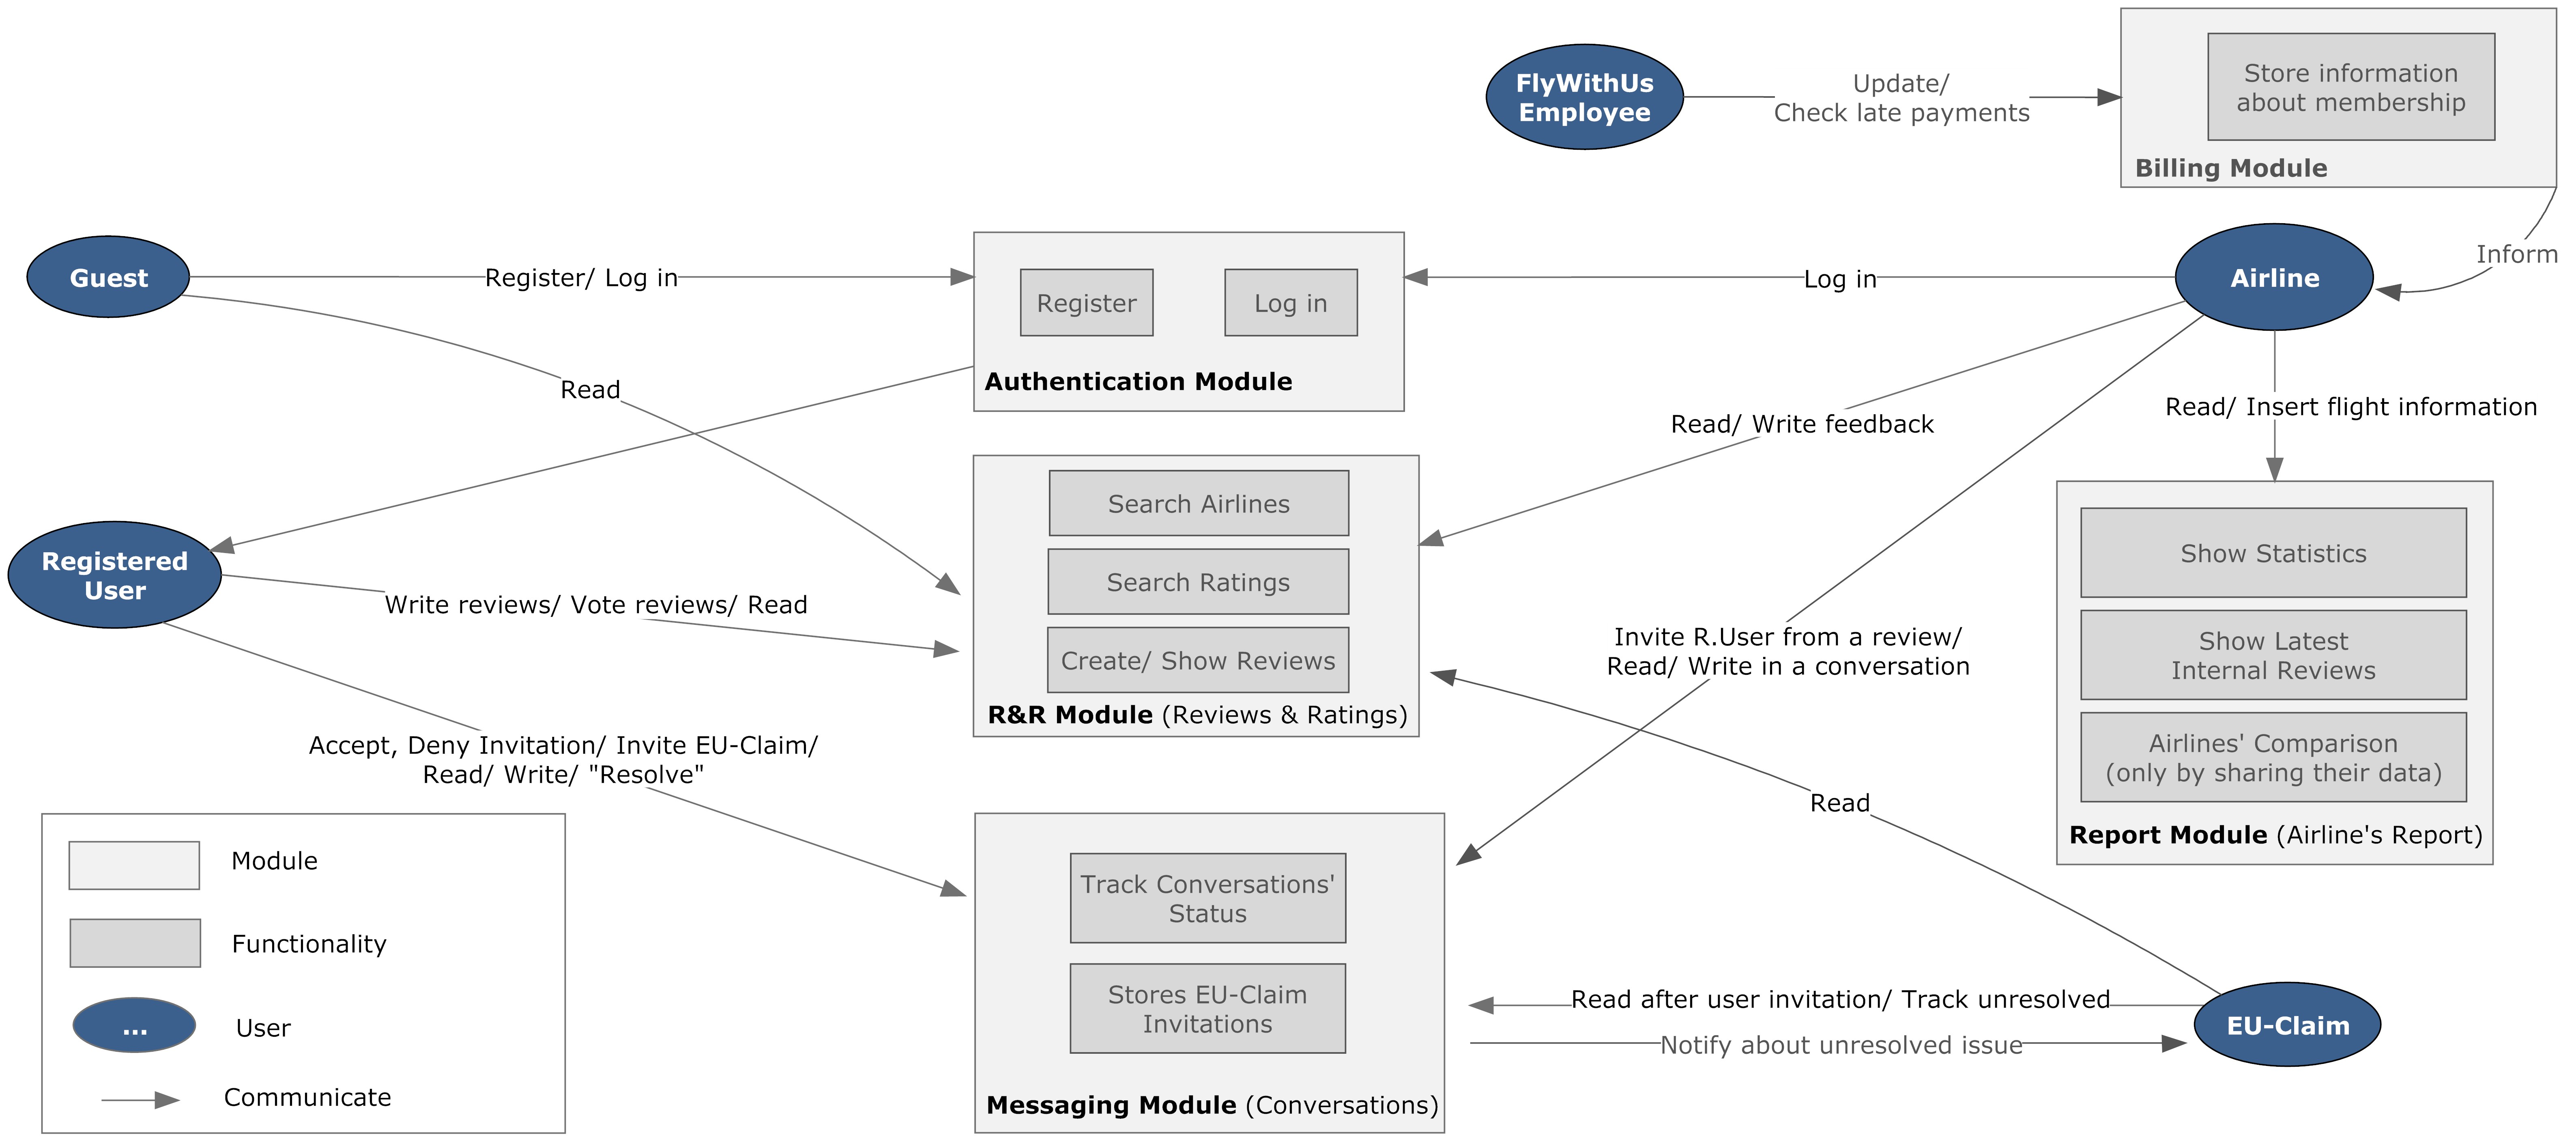
\includegraphics[width=600px]{Functional_Viewpoint.jpg}
\caption{Functional Viewpoint}
\label{fig:functional}
\end{figure}
\end{landscape}

The functional viewpoint (Fig.~\ref{fig:functional}) illustrates the functionality supported by the system and its connections to the users. The direction of the arrows shows the initiator of its connection, for example EU-Claim can monitor a conversation and the system notifies EU-Claim about an issue that has been unresolved for a configurable period of time. The functionalities that are based in the same entities of the system are grouped together to help the reader understand their connections. For example, all the functionalities 
 provided only to airlines are included in a {\em report} as a result these functionalities are grouped in the {\em Report System}. The association between the subsystems presented in the viewpoint and the functional requirements listed in table~\ref{} is shown in table~\ref{tab:associateSysReq}.

\begin{longtable}{| l | l | l |}
\label{tab:associateSysReq}
\textbf{Requirement} & \textbf{System} & \textbf{Users} \\ \hline
Show ratings & Review System & Guests, Registered Users  \\ \hline
Post/Read/Search/Vote!!!! & Review System & Registered Users \\ \hline
Messaging & Messaging System & Registered Users, Airlines, EUC\\ \hline
Reporting  & Reporting System & Airlines \\ \hline
Flight Information & Reporting System & Airlines  \\ \hline
Statistics & Reporting System & Airlines \\ \hline 

\end{longtable}

 Furthermore, the viewpoint also presents the availability of the functionalities to each user group and the communication between these groups through the system. For instance, a guest can register or log in the system and  become a registered user, or an airline can invite a user to a private conversation in order to resolve a potential complaint; then the user can accept the invitation and he/ she can 
 also invite EU-Claim to monitor their conversation to ensure the integrity of this process.

